\newcommand{\BL}{D}
\newcommand{\CH}[1]{c(#1)}
\newcommand{\LB}[1]{l_{#1}}
\newcommand{\LBh}{n_l}
\newcommand{\NV}{N}
\newcommand{\RBh}{n_r}
\newcommand{\RN}{\psi}
\newcommand{\RNALL}{\Psi}
\newcommand{\SD}{\omega}
\newcommand{\SDALL}{\Omega}
\newcommand{\TO}{T^\SD}
\newcommand{\TR}{T^\RN}
\newcommand{\TRO}{\TR_{\SD}}
\newcommand{\bl}{\delta}
\newcommand{\child}[2]{#1_{#2}}
\newcommand{\defeq}{=}
\newcommand{\la}{\lambda_a}
\newcommand{\lb}{\lambda_b}
\newcommand{\leaf}{\otimes}
\newcommand{\tO}{t^\SD}

\newtheorem{conjecture}{Conjecture}
\newtheorem{corollary}{Corollary}
\newtheorem{lemma}{Lemma}
\newtheorem{theorem}{Theorem}

%% START DUAL-BIRTH CHAPTER
\chapter{\dualbirthtitle}
\label{chap:dualbirth}
\clearpage

Models of tree evolution have mostly focused on capturing the cladogenesis processes behind speciation. Processes that derive the evolution of genomic elements, such as repeats, are not necessarily captured by these existing models. In this paper, we design a model of tree evolution that we call the dual-birth model, and we show how it can be useful in studying the evolution of short \textit{Alu} repeats found in the human genome in abundance. The dual-birth model extends the traditional birth-only model to have two rates of propagation, one for active nodes that propagate often, and another for inactive nodes, that with a lower rate, activate and start propagating. Adjusting the ratio of the rates controls the expected tree balance. We present several theoretical results under the dual-birth model, introduce parameter estimation techniques, and study the properties of the model in simulations. We then use the dual-birth model to estimate the number of active \textit{Alu} elements and their rates of propagation and activation in the human genome based on a large phylogenetic tree that we build from close to one million \textit{Alu} sequences.

\section{Introduction}
Phylogenetic trees can be used to study the evolution of not just species, but of any sequence that evolves. For example, multi-copy gene families~\cite{Page1997,Finn2014}, cancer genomes~\cite{Nowell1976,El-Kebir2016}, antibodies~\cite{Litman1993,Robinson2015,Safonova2015}, segmental duplicates~\cite{Bailey2006,Jiang2007}, and long or short interspersed nuclear elements~\cite{Dewannieux2003} are all biological sequences that evolve, and many of these evolve \textit{within} the genome of a single species. The process of diversification for many evolving entities can be characterized by propagation: an original copy of a sequence creates a new copy, and the two copies evolve independently by accumulating mutations. Phylogenetics provides a natural framework for studying such processes, but several challenges present themselves.

Given sufficiently long sequences and assuming our models of sequence evolution are reasonably accurate, we can recover the phylogenetic trees from sequence data with high accuracy~ \cite{Felsenstein2003,Roch2010}. However, unlike species-tree reconstruction, in which the entire genome can be used, reconstructing phylogenies of gene families, repeats, or antibodies is limited by the length of the evolving entity. As a result, high levels of uncertainty are to be expected in trees reconstructed from these types of sequences. These inherent limitations make accurate modeling of underlying processes crucial, perhaps even more so than species-tree reconstruction.

Models of tree evolution describe probability distributions over the space of tree shapes ~\cite{Yule1925,Brown1994,Aldous2001} and are useful in several ways. They can be used as the prior distribution in a Bayesian inference~\cite{Drummond2007,Mooers2012,Sayyari2016}. They can also generate null distributions describing certain neutral evolutionary process, which may then be rejected by trees inferred from the data~\cite{Guyer1991,Kirkpatrick1993,Agapow2002}. Moreover, the diversification parameters are inherently of interest to the biologist~\cite{Morlon2014}. Two well-known models of tree evolution are Yule (birth-only), in which each branch splits by a Poisson process with a constant rate, and birth-death, in which, in addition to birth, branches can go extinct with a constant rate. Each of these models have limitations and have inspired the development of several alternative models~\cite{Aldous1996,Steel2001,Ford2005,Blum2006,Jones2011,Maddison2007}.

A main feature of a tree evolution model is the expected tree shape, especially the tree balance (Fig.~\ref{fig:dualbirth-model}). The Yule model generates relatively balanced trees~\cite{McKenzie2000}, more so than typically seen in phylogenetic trees~\cite{Blum2006}. Some systems, such as certain viruses, are especially known to have very unbalanced trees~\cite{Volz2013}. Most models of evolution are exchangeable, meaning that, after a split, the two branches are indistinguishable. When evolution works in a series of propagation events (i.e., where an element copies itself), there is a natural way in which one of the child branches corresponds to the parent branch~\cite{Lambert2013}. The new copy may have properties that are different from the original branch, and as a result, non-exchangeable models may be more appropriate. For example, the new child may be initially incapable of propagation until it \textit{activates}. In such situations, the tree will tend to be unbalanced. In the limit, if every new child is impotent, one would expect a {\em caterpillar}-like tree (Fig.~\ref{fig:dualbirth-model}).

In this paper, we study a non-exchangeable extension of the Yule model, which we name the dual-birth model. Each branch will split with one of two available rates. Branches that correspond to elements that have in the past propagated are considered \textit{active} and have a high rate of future propagation, whereas  branches that have never propagated are considered \textit{inactive}. With some rate, the Unlike some previous models (e.g. BiSSE~\cite{Maddison2007}), after every birth event, one of the two children inherits the parent's rate while the other child has the opposite rate (i.e., the model is asymmetric in the terminology of Lambert and Stadler (2013)~\cite{Lambert2013}). For this dual-birth  model, we describe methods for sampling the tree distribution, derive probability distributions on the tree space, compute the expectation of various tree statistics, and introduce methods of estimating the model parameters from data. In extensive simulations, we study the behavior of the model and our estimators. We then use the model to study the evolution of \textit{Alu} elements in the human genome.

\textit{Alu} elements are a family of \glspl{SINE}, each approximately 300bp long, that abound in the genomes of supraprimates and that retrotranspose via \gls{RNA} polymerase III-encoded \glspl{RNA}~\cite{Dewannieux2003}. There are approximately one million \textit{Alu} elements in the human genome, meaning they comprise roughly 10\% of the human genome. Although \textit{Alu} elements have no known biological function of their own~\cite{Schmid2003}, studying and understanding their retrotransposition in the genome can provide key insight into their contributions to genetic disease~\cite{Deininger1999} as well as useful information in the study of supraprimate evolution~\cite{Stoneking1997,Singer2003,Watkins2003}.

A topic of interest regarding \textit{Alu} elements is the number and identity of repeats that are capable of propagating through retrotransposition~\cite{Cordaux2004,Liu2009,Konkel2015}. Various hypotheses range from the single source model to the transposon model, where all elements are assumed to be equal in their ability to propagate~\cite{Cordaux2004}. We approach this question using phylogenetics and the dual-birth model. We build a tree for close to one million \textit{Alu} elements. Using the properties of the dual-birth model, we estimate the number of \textit{Alu} elements that have been active and estimate the rates of \textit{Alu} propagation and activation.

\section{Materials and Methods}
\subsection{Dual-Birth Model}
The dual-birth model is similar to the Yule process, but unlike Yule, it is not \textit{exchangeable}, meaning that left and right branches are not generated using identical processes. The dual-birth model is parameterized by two birth parameters: $\la$ and $\lb$. The generative process starts with a single root node, which immediately splits into two child branches \textit{left}, denoted by $a$,  and \textit{right}, denoted by $b$. Further birth events occur on each child branch according to a Poisson process with the constant rate $\la$ on branch $a$ and the constant rate $\lb$ on branch $b$. Thus, \textit{left} and \textit{right} are governed by different rates. Each new node becomes the root of an identical process. The process can be terminated at any point in time. This generates an unlabeled \textit{ordered}, also known as oriented~\cite{Lambert2013}, tree: each branch is labeled as either \textit{left} or \textit{right} (Fig.~\ref{fig:dualbirth-model}a). We define $r=\la/\lb$ and $\lambda=\la+\lb$, which together identify $\la$ and $\lb$. When $r=1$, the dual-birth process is reduced to the Yule process
with a rate of $\lambda/2$.

\subsubsection{Active/inactive elements}
Consider a tree in which each branch corresponds to some entity, and the right child of any branch corresponds to the same entity as the parent. Thus, each split is a propagation of the parent entity. Moreover, entities are either \textit{active} or \textit{inactive}. A branch is active if it has produced an offspring before and is otherwise considered inactive. The right child of any branch is always active while the left one is  inactive. Active entities  propagate with rate $\lb$ (for ``birth''), and inactive entities activate and simultaneously propagate with rate $\la$ (for ``activation''). Note that activation and the first propagation occur together (an alternative model could be that nodes activate mid-branch and wait for a birth event). Once an entity activates, it remains active (thus, there is no deactivation).

The dual-birth model can easily capture this scenario. If $r=1$ (i.e., the Yule model), active and inactive nodes have the same rates of birth, and thus, their difference is inconsequential. When $r<1$, new entities activate (i.e., propagate for the first time) with a rate $\la$ that is lower than the rate $\lb$ with which nodes that are already active propagate (Fig.~\ref{fig:dualbirth-model}b). Allowing $\la > \lb$ would result in $r > 1$, which yields a model that is non-identifiable with the model that has rate $1/r$. Setting $r>1$ would correspond to a scenario where the rate of propagation \textit{reduces} after the first activation, and we don't know of any scenario that justifies such reductions. Thus, our model defines $\la\leq\lb$ to remain identifiable.

One application of the dual-birth model is to study \textit{Alu} elements, though the model may prove useful for other systems, such as retroviruses or gene families. Each \textit{Alu} element appears at a specific position in the genome, and via retrotransposition, it can create a new copy of itself elsewhere in the genome, leading to a split in the repeat evolutionary tree. Each branch of the tree can thus be labeled by a position in the genome, which is the site at which the corresponding element resides. One child branch inherits the same position as the parent (and is thus active), and the other branch is the new copy, which is assumed to be initially inactive. The inactive state captures the observation that most \textit{Alu} elements don't propagate~\cite{Batzer2002}. The model allows for the chance that some inactive elements become active and start propagating, perhaps due to mutations or due to changes in their genomic context.

\subsubsection{Tree balance}
The Yule model generates balanced trees, more so than trees typically found in phylogenetic databases~\cite{Guyer1991,Blum2006,Jones2011}. Similar to several other models of tree evolution~\cite{Aldous1996,Blum2006,Maddison2007}, the dual-birth model provides a natural way to control tree balance (we provide an extensive comparison to other models in the Discussion section). Consider an extreme case in which only one element is ever active. The resulting tree is a caterpillar, which will include only one cherry (an internal node is called a cherry if both of its children are leaves, i.e., terminal nodes). This outcome can be naturally achieved in dual-birth by setting $\la=0$ (i.e., $r=0$). When we expect to have many more inactive nodes than active nodes, we would still expect to see an unbalanced tree with few cherries. This outcome, too, can be achieved by a natural choice of $\la\ll\lb$, which results in $r\ll 1$. As $r$ increases, the tree becomes gradually more balanced (Fig.~\ref{fig:dualbirth-model}b). With $r=1$, the tree is as balanced as expected under the Yule model.

\begin{figure} % FIGURE 1 IN ORIGINAL PAPER
\centering
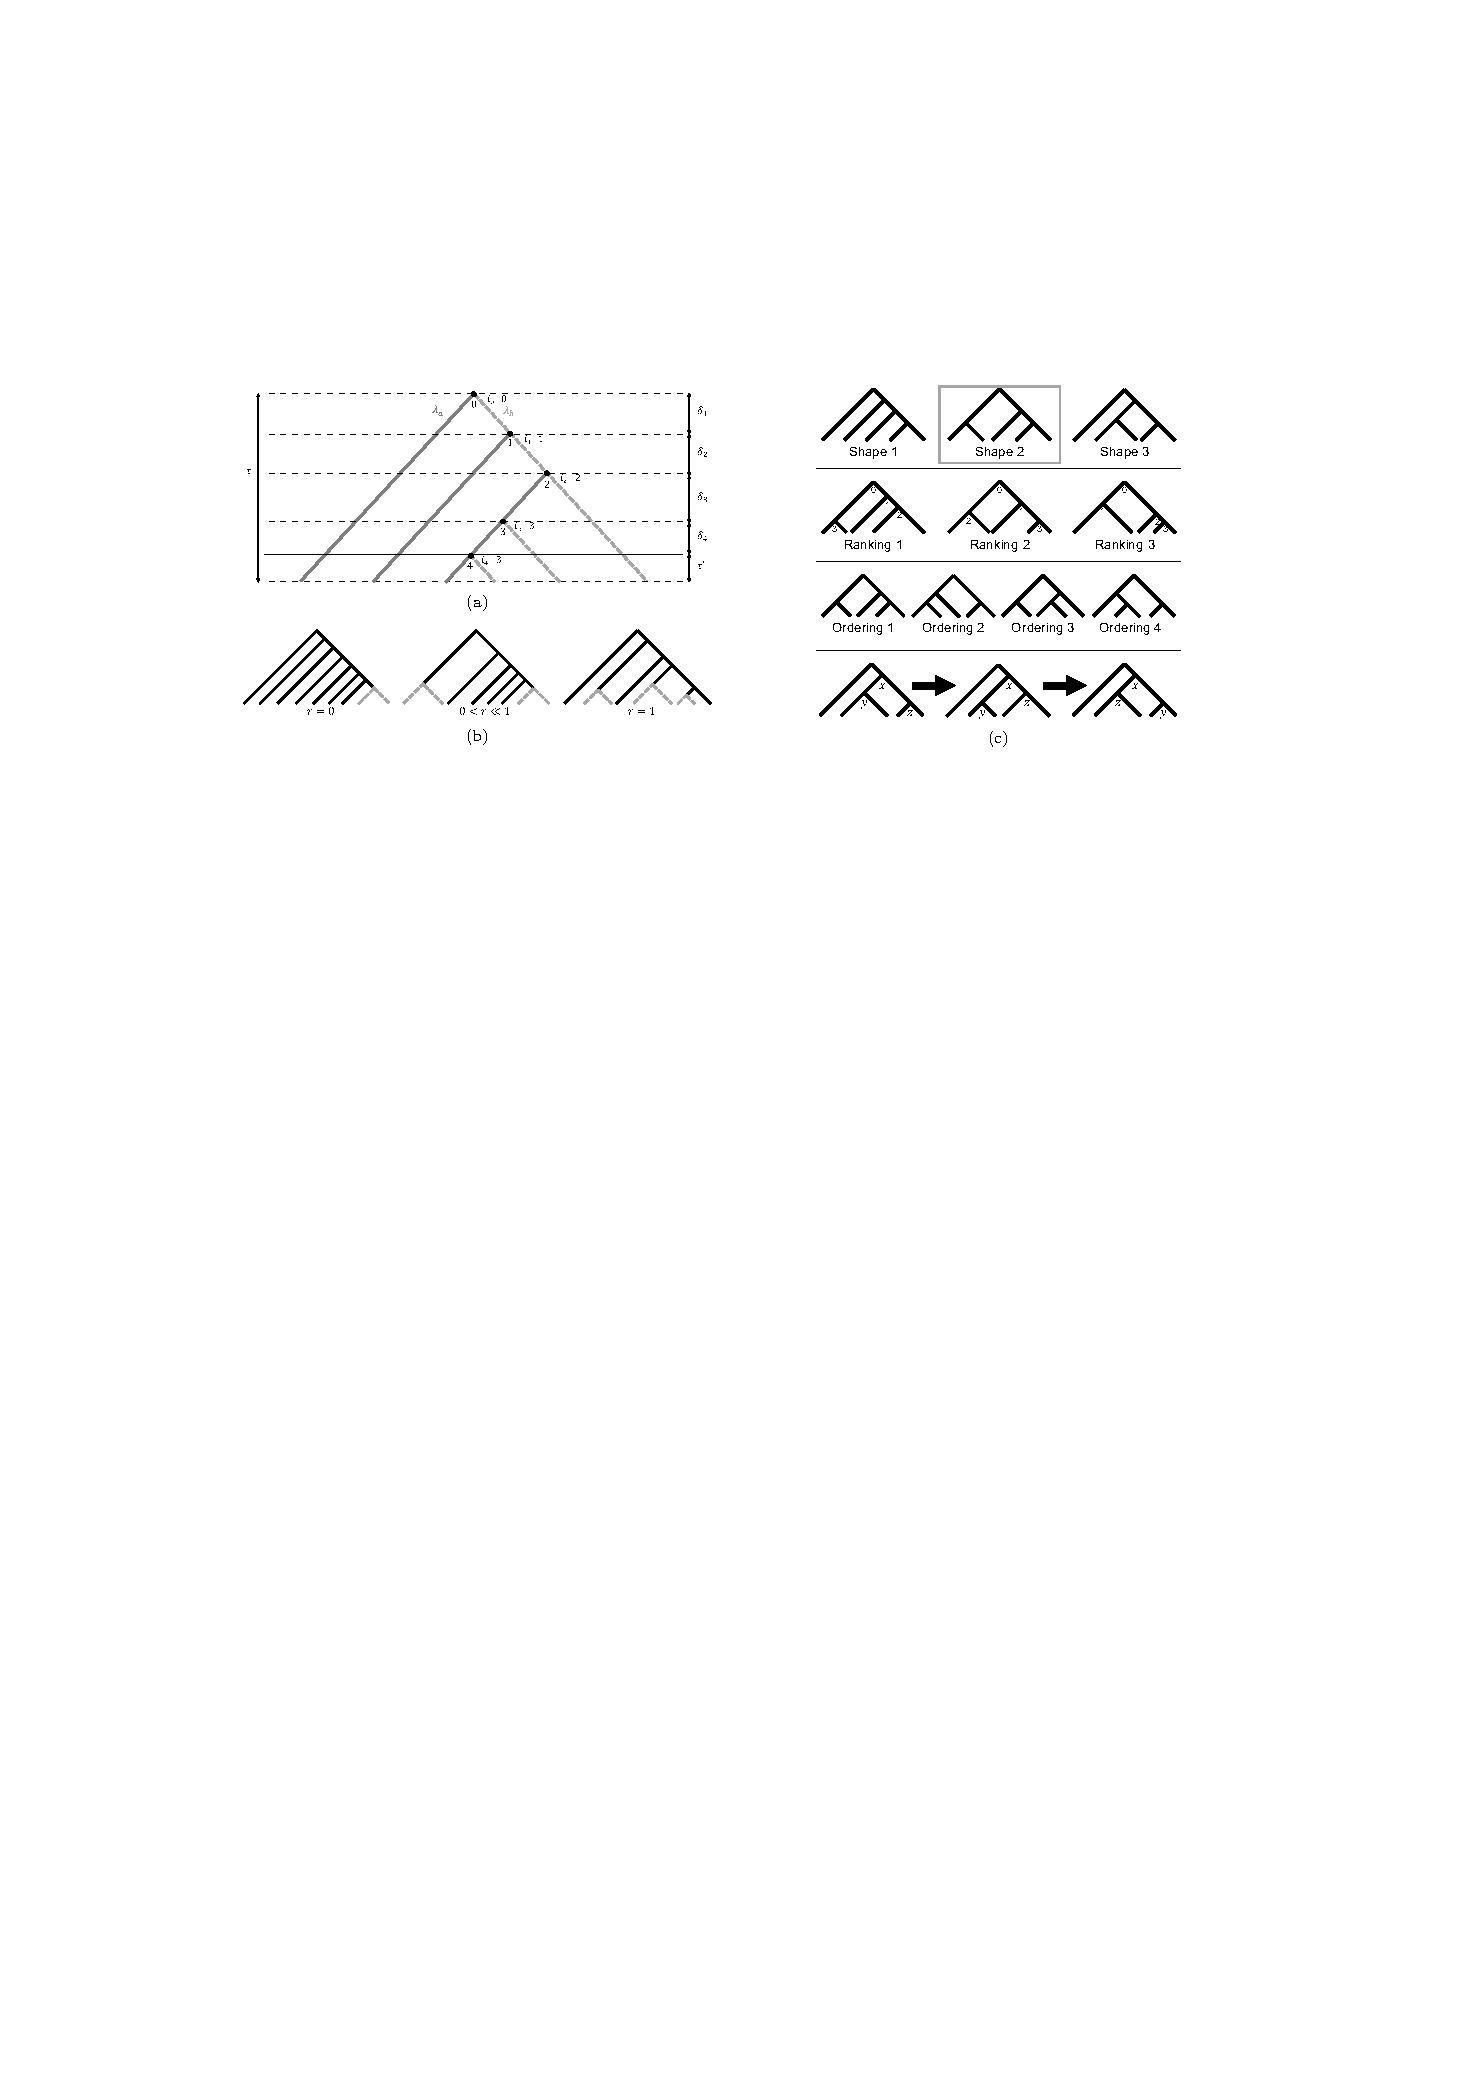
\includegraphics[width=\textwidth]{figs/dualbirth-model}
\caption[Dual-birth model]
{Dual-birth model. (a) A caterpillar tree with one cherry (node 4). The tree is generated by the dual-birth model; right branches (dashed light gray) are sampled from the Poisson process with rate $\lb$, and left branches (solid dark gray) are sampled with rate $\la$. Internal nodes are ranked by distance to the root (ranks shown below nodes), and the tree is divided into time intervals between consecutive nodes. (b) With $r=\la/\lb=0$, only caterpillar trees can be generated; as r increases toward $1$, the tree becomes more balanced and thus has more cherries (dashed light gray). (c) All three possible tree shapes with five leaves are shown on top; the second row shows $\RNALL$, all possible rankings of tree shape 2; the third row shows $\SDALL$, all orderings of tree shape 2. The last row demonstrates that, starting from a ranked ordered tree, one change of ranking followed by a change of ordering results in a tree identical to the original tree.}
\label{fig:dualbirth-model}
\end{figure}

\subsection{Theoretical Properties of the Dual-Birth Model}\label{sec:dualbirth-meth}
\subsubsection*{Notations and definitions}
A connected \gls{DAG} with no undirected cycles defines a tree. We only consider binary trees in which all nodes either have outdegree zero (leaves) or two (internal nodes). Two trees are considered to have the same \textit{shape} if there exists a one-to-one mapping between their nodes such that the head and tail of every edge in one tree map to the head and tail of exactly one edge in the other tree. In this paper, we care about the space of distinct tree shapes. In the tree-shape space, leaves are not distinguished (i.e., a tree shape is unlabeled). For simplicity of presentation, we represent a tree shape on $n$ leaves using $T=(V,E)$, where $V$ is the set of $n-1$ \textit{internal} nodes and $E$ is the set of internal edges $(u,v)$ from parent node $u$ to child node $v$. Note that terminal edges (connecting internal nodes to leaves) and leaves are not part of $E$ and $V$, and as such, are implicit in the $T$ formulation (each internal node has to have outdegree two). We use $\child{u}{1}$ and $\child{u}{2}$ to denote the children of $u$, and we use $\leaf$ to denote a generic unlabeled leaf. Note that $T$  defines a \gls{POSET} on $V$.

Recall a node $v\in V$ is called a cherry if both of its children are leaves. A tree shape is called \textit{caterpillar} if it has only one cherry (Fig.~\ref{fig:dualbirth-model}a); in contrast, a fully-balanced tree has exactly $n/2$ cherries. The number of cherries of a tree is denoted as $\CH{T}$.

Let $\NV\defeq\{0,1,\ldots, n-2\}$. A bijective function $\RN:V\mapsto\NV$ is a ranking of a tree $T=(E,V)$  if for each edge $(u,v)\in E$, we have $\RN(u)<\RN(v)$. A \textit{ranked tree shape} is defined as $\TR\defeq (T,\RN)$. Each ranking is a topological sorting of the tree (i.e., is a linear extension of the \gls{POSET} defined by the tree shape). We use $\RNALL(T)$ to denote the set of all possible rankings of the tree shape $T$ (Fig.~\ref{fig:dualbirth-model}c).

An \textit{ordered tree shape} is a tree shape in which left and right child nodes are distinguished (i.e., the tree is oriented). More precisely, $\SD:V\mapsto\{0,1\}$  is a valid order for a tree shape $T$ iff $\SD(\child{u}{1})+\SD(\child{u}{2})=1$ for every $(u,\child{u}{1}),(u,\child{u}{2})\in E$ and $\SD(r)=1$ for the root node $r$. We call $v$ a left child/node when $\SD(v)=0$ and otherwise call it a right child/node. A branch leading to a left (right) child is called a left (right) branch. An ordered tree shape is denoted by $\TO\defeq(T,\SD)$. Note that, in this definition, leaves are not directly assigned a left/right side. Leaves below a cherry are indistinguishable; leaves that are sister to internal nodes are considered to have the opposite side of their sibling. For example, in Figure~\ref{fig:dualbirth-model}a, the leaf directly below the root is considered a left node because its sister, the node ranked 1, is a right node. Also, $\SDALL(\TR)$ denotes the set of all possible orderings that are valid for $\TR$ (Fig.~\ref{fig:dualbirth-model}c).

A ranked ordered tree shape is defined by $\TRO\defeq(T,\RN,\SD)$. For ease of notation, we define $\SD_i\defeq\SD\left(\RN^{-1}(i)\right)$ (the order of the node ranked $i$). For $0<i<n$ and the ranked ordered tree $\TRO$, we define $\LB{i}(\TRO)\defeq1+\sum_{k=1}^{i-1}\SD_k$ and it is easy to show that $\LB{i}(\TRO)$ gives the number of left branches $(u,v)$ with $\SD(u) < i$ and $\SD(v) \geq i$. In other words, $\LB{i}(\TRO)$ gives the number of left terminal branches if the tree $\TRO$ is terminated at the time when node $i$ is created. Where clear by the context, we simply write $\LB{i}$ (Fig.~\ref{fig:dualbirth-model}a). We define $\LBh\defeq\LB{n-1}$ and $\RBh\defeq n-\LBh$; these definitions can be intuitively considered to show the number of left and right terminal branches, respectively, if we assign an order to all terminal branches (e.g. $\RBh=\LBh=3$ in Fig.~\ref{fig:dualbirth-model}a).

We refer to a tree shape with ultrametric branch lengths as a weighted shape. A weighted shape is defined by $t\defeq(T,\bl,\tau)$, where $\bl:E\mapsto\mathbb{R}$ gives the length of internal branches and $\tau$ gives the distance from the root to all leaves; note that $\tau$ has to be larger than the largest distance to the root from any internal node. Node ages define a unique ranking on any weighted shape. A weighted shape $t$ can also be assigned an order, $\SD$, and will be denoted by $\tO$. For $e=(u,v)\in E$, we refer to  $\bl(e)$ by $\bl_i$ where $i={\RN(v)}$ (e.g. $\bl_1\ldots\bl_4$ in Fig.~\ref{fig:dualbirth-model}a).

\subsubsection{Probability distributions}
We now derive probability distributions on tree shapes conditioning on fixed $n$. Here we give the main results and provide the proofs in Section~\ref{sec:dualbirth-proofs}.

\begin{theorem}\label{thm:TRO}
Let $X$ be a random variable (r.v.) over ordered ranked tree shapes and distributed according to the dual-birth model with parameter $r=\la/\lb$. Then, 
\begin{equation}\label{eq:orts}
\Pr(X=\TRO;n) = \frac{r^{\RBh-1}}{\prod_{i=1}^{n-2} \big((r-1)\LB{i}+i+1\big)}
\end{equation}
\end{theorem}

Computing Equation~\ref{eq:orts} simply requires knowing the number of right leaves ($\RBh$) and the number of its left branches if the tree is terminated at each node $i$ ($\LB{i}$); all of these can be computed in time $O(n)$ for an ordered tree. Figure~\ref{fig:dualbirth-tree-prob-dists} shows the perfect match between Equation~\ref{eq:orts} and observed frequencies in simulations for all ranked ordered tree shapes with $n=6$ and shows that, with $r\ll1$, the caterpillar tree shape has a high probability.

The left/right order of nodes cannot be estimated from sequence data, and thus, it would be more useful to compute the probability distribution over unordered ranked tree shapes. Since all orderings of a {\em ranked} tree are distinct, the probability of a ranked tree simply needs to marginalize over all possible orderings. Thus,
\begin{corollary}
For $Y$, an r.v.\ over ranked tree shapes with $n$ leaves and distributed according to the dual-birth model,
\begin{equation}\label{eq:rts}
\Pr(Y=\TR;n) = \sum_{\SD\in\SDALL(\TR)} \Pr(\TRO)
\end{equation}
where $\SDALL$ gives the set of all orderings of $\TR$.
\end{corollary}

This computing requires
an exponential number of 
computations to iterate all orderings (the recursive formula for that iteration is given
 in the supplement, Eq. S5. %~\ref{sup:eq:sdall}).
%%%%%%%%in \ref{sup:eq:sdall}. 
Whether efficient
algorithms for computing this probability 
exist is unclear to us. 
See Figure S1 %~\ref{fig:rankedordered}
for an example distribution
and matching simulations.

%% END DUAL-BIRTH CHAPTER